% \documentclass[12pt, oneside]{book}

\chapter{Coriolis force and Ekmann Balance}
\label{ch:coriolis}

\begin{tabular}{ll}
    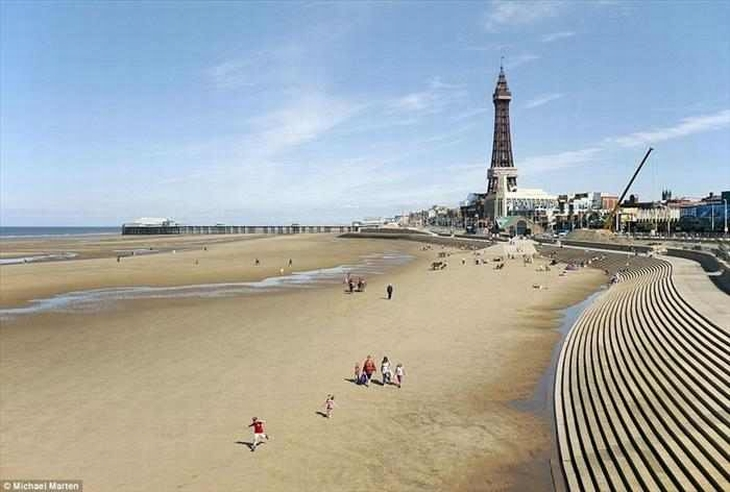
\includegraphics[width=3.2in]{figs/Waves/LowTide.jpg} & 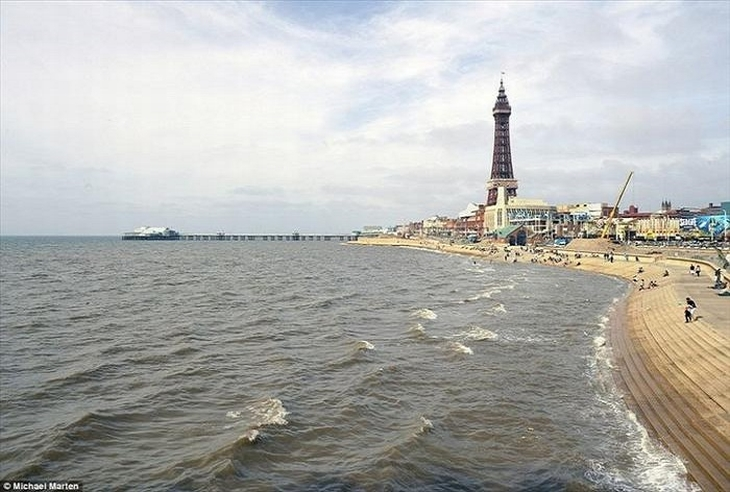
\includegraphics[width=3.2in]{figs/Waves/HighTide.jpg}
\end{tabular}

The large-scale circulation of the ocean occurs on spatial scales spanning the size of ocean basins and temporal scales of hours to decades.  On these scales, the earth's rotation matters at leading order to the dynamics of the motions, via an apparent force we call the \Wikiref{Coriolis force}.

\section{Quick review of forces and apparent forces}

First, its helpful to quickly review forces, and then discuss what we mean by an \Wikiref{apparent force}.  

\Wikiref{Newton's second law} says that the rate of change of a body's velocity ($\mathbf{u}$) is proportional to the \emph{net} force exerted on it:
\begin{equation}
    \sum{\mathbf{F}_i} = m \frac{d \mathbf{u}}{dt}
\end{equation}
where we have used bold to remind ourselves that the \emph{direction} of the force matters.  As with concentrations, in fluid mechanics it is more natural to consider force per mass, or 
\begin{equation}
    \sum{\mathbf{a}_i} = \frac{d \mathbf{u}}{dt}.
\end{equation}

It is possible for a body to have forces being exerted on it, but those forces be in ``balance'' so that the acceleration of the body is zero (or approximately zero).  A common example from physics classes is a falling body that has reached its \Wikiref{terminal velocity}, which is a balance between the force of gravity pulling the body down, and friction resisting the downward motion:
\begin{equation}
    \frac{dw}{dt} = -g + Fr \approx 0
\end{equation}
where $w$ is the vertical component of velocity, and $Fr$ is the wind friction at the terminal velocity (\fref{fig:TermVel}).  

\begin{marginfigure}
    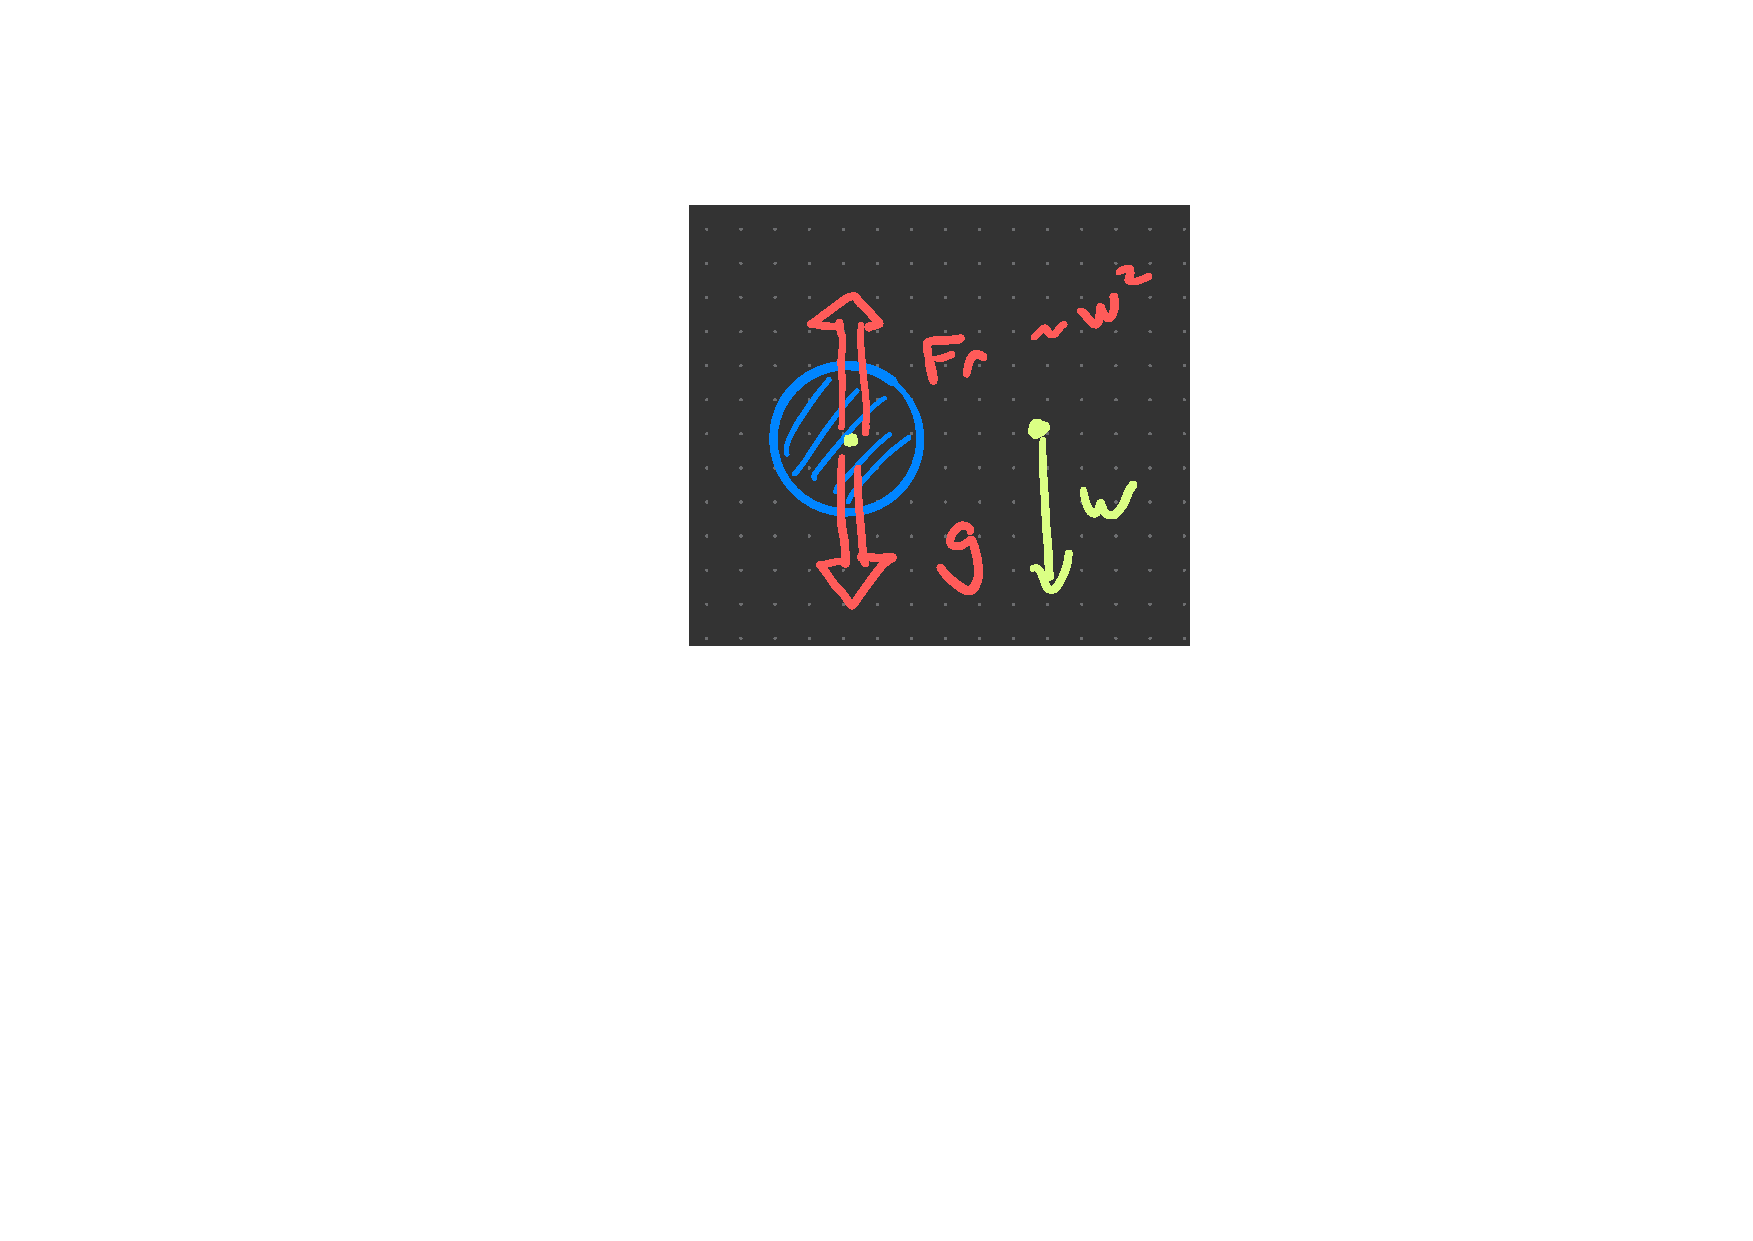
\includegraphics[width=1.7in]{figs/Coriolis/TermVel}
    \caption{Sketch of terminal velocity force balance.  In balance, the gravity force $g$ is equal and opposite to the friction force ($F_r$).}
    \label{fig:TermVel}
\end{marginfigure}

The idea of an \Wikiref{Apparent force} or \Wikiref{Inertial Force} is not 

%%% Local Variables:
%%% mode: latex
%%% TeX-master: t
%%% End:
